

%% this section contains XX problems
%%----------------------------------------


%% Jacobs 5 steps to a 5
%%------------------------------
\element{AP}{
\begin{question}{Jacobs-Q10}
    Two identical small balls are moving with the same speed
        toward a brick wall.
    After colliding with the wall, ball 1 sticks to the wall
        while ball 2 bounces off the wall, moving with almost
        the same speed that it had initially.
    Which ball experiences greater impulse?
    \begin{multicols}{3}
    \begin{choices}
        \wrongchoice{ball 1}
      \correctchoice{ball 2}
        \wrongchoice{Both experiences the same impulse}
        \wrongchoice{The answer cannot be determined unless
            we know the time of collision.}
        \wrongchoice{The answer cannot be determined unless
            we know the force each ball exerts on the wall.}
    \end{choices}
    \end{multicols}
\end{question}
}

\element{AP}{
\begin{question}{Jacobs-Q11}
    Ball $A$ moves to the right with a speed of \SI{5.0}{\meter\per\second};
        Ball $B$ moves to the left with speed \SI{2.0}{\meter\per\second}.
    Both balls have mass \SI{1.0}{\kilo\gram}.
    What is the total momentum of the system consisting
        only of balls $A$ and $B$?
    \begin{multicols}{3}
    \begin{choices}
        \wrongchoice{\SI{7.0}{\newton\second} to the right}
      \correctchoice{\SI{3.0}{\newton\second} to the right}
        \wrongchoice{zero}
        \wrongchoice{\SI{7.0}{\newton\second} to the left}
        \wrongchoice{\SI{7.0}{\newton\second} to the left}
    \end{choices}
    \end{multicols}
\end{question}
}

\element{AP}{
\begin{question}{Jacobs-Q12}
    Momentum of a system always remains constant.
    However, in a collision between two balls,
        a ball's momentum might change from, say,
        \SI[retain-explicit-plus]{+1}{\kilo\gram\meter\per\second}
        to \SI[retain-explicit-plus]{-1}{\kilo\gram\meter\per\second}.
    How can this be correct?
    \begin{multicols}{3}
    \begin{choices}
        \wrongchoice{It is \emph{not} correct.
            Momentum conservation means that the momentum
            of an object must remain the same.}
        \wrongchoice{A force outside the two-ball system must have acted.}
        \wrongchoice{Friction is responsible for the change in momentum.}
      \correctchoice{Although one ball's momentum change,
            the momentum of \emph{both} balls in total remained the same.}
        \wrongchoice{Momentum is conserved because the magnitude of
            the ball's momentum remained the same.}
    \end{choices}
    \end{multicols}
\end{question}
}


%% 2004-APB
%%------------------------------
\element{AP}{
\begin{question}{2004-APB-Q09}
    An empty sled of mass $M$ moves without friction across a frozen pond
        at speed $v_0$.
    Two objects are dropped vertically into the sled one at a time:
        first an object of mass $m$ and then an object of mass $2m$.
    Afterward the sled moves with speed $v_f$.
    What would be the final speed of the sled if the objects were dropped
        into it in reverse order?
    \begin{multicols}{3}
    \begin{choices}
        \wrongchoice{$v_f/3$}
        \wrongchoice{$v_f/2$}
      \correctchoice{$v_f$}
        \wrongchoice{$2 v_f$}
        \wrongchoice{$3 v_f$}
    \end{choices}
    \end{multicols}
\end{question}
}

\element{AP}{
\begin{question}{2004-APB-Q40}
    Two objects, $A$ and $B$, initially at rest, are ``exploded'' apart by
        the release of a coiled spring that was compressed between them.
    As they move apart, the velocity of object $A$ is \SI{5}{\meter\per\second}
        and the velocity of object $B$ is \SI{-2}{\meter\per\second}.
    The ratio of the mass of object $A$ to the mass of object $B$,
        $m_A/m_B$, is
    \begin{multicols}{3}
    \begin{choices}
        \wrongchoice{\num{4/25}}
      \correctchoice{\num{2/5}}
        \wrongchoice{\num{1/1}}
        \wrongchoice{\num{5/2}}
        \wrongchoice{\num{25/4}}
    \end{choices}
    \end{multicols}
\end{question}
}

\element{AP}{
\begin{question}{2004-APB-Q63}
    The two blocks of masses $M$ and $2M$ shown below initially travel
        at the same speed $v$ but in opposite directions.
    The collide and stick together.
    \begin{center}
        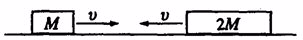
\includegraphics[keepaspectratio]{2004-APB-Q63}
    \end{center}
    How much mechanical energy is lost to other forms of energy
        during this collision?
    \begin{multicols}{3}
    \begin{choices}
        \wrongchoice{Zero}
        \wrongchoice{$\dfrac{M v^2}{2}$}
        \wrongchoice{$\dfrac{3 M v^2}{4}$}
      \correctchoice{$\dfrac{4 M v^2}{3}$}
        \wrongchoice{$\dfrac{3 M v^2}{2}$}
    \end{choices}
    \end{multicols}
\end{question}
}

